% Implementation Results -- handbook section 3

\subsection{Training behaviour}
\label{subsec:results-1}
% Required: Loss and metric curves; selected checkpoint; overfitting or underfitting; training time; implementation issues and fixes.

Figure~\ref{fig:curves} shows the learning curves, each averaged over three seeds. The ordering
visible at epoch 30 is already established by epoch 10 and does not cross afterwards.

\begin{figure}[H]
    \centering
    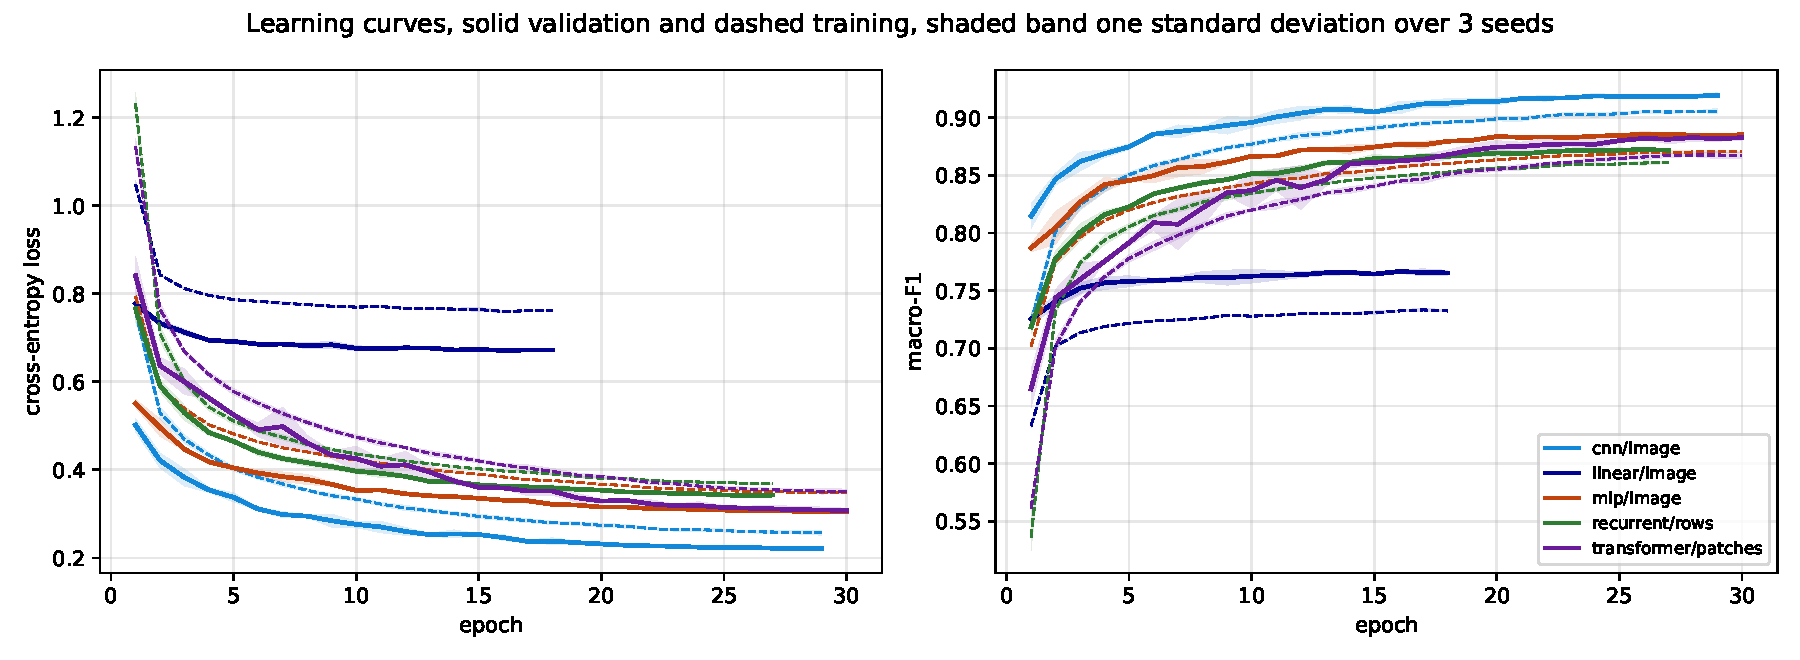
\includegraphics[width=\textwidth]{images/learning_curves.pdf}
    \caption{Learning curves per architecture, averaged over three seeds.}
    \label{fig:curves}
\end{figure}

Validation scores better than training, not worse: for the CNN, MLP and Linear baseline,
validation loss is below training loss and validation macro-F1 above it at every epoch of every
seed, and the Transformer and GRU agree until individual seeds cross over in the final third.
This is not leakage. Augmentation and dropout are active in the training pass only, so training
metrics are measured on a deliberately harder task; the gap is the cost of that regularization.

None of the five overfits: validation loss is still at its minimum in the final epoch for every
architecture, exceeding it by at most $0.0008$. The Linear baseline is the one clear case of
underfitting, plateauing near $0.77$ macro-F1 while its training loss stays high. Early stopping
fired only for that baseline, at 24.3 epochs on average; the other four ran the full 30 with the
best epoch between 25.3 and 27.3, so the budget was adequate but not generous.

Three implementation faults were found and fixed, each of which would have corrupted the
comparison. The run directory was written before the normalization statistics were computed, so
the recorded configuration did not describe the run. The loader then recomputed those statistics
instead of reusing the recorded ones, found by tampering with the recorded value and seeing it
silently overwritten. Per-run metrics were rounded before averaging across seeds, inflating the
measured standard deviation by up to $26.8\%$.

\subsection{Quantitative results}
\label{subsec:results-2}
% Required: Primary and secondary metrics; parameter counts; training and inference time; configurations; mean and standard deviation over multiple runs where feasible.
% Also required: Section 12.1: accuracy, macro-F1, parameter count, training time, inference time.

Table~\ref{tab:results} reports every mandatory comparison quantity as a mean over seeds $0$,
$1$ and $2$ with one standard deviation. Inference time is per image at batch size 1, and the
fifteen runs were trained consecutively on the one idle machine of Table~\ref{tab:protocol}, so
the times compare with each other but do not transfer. Accuracy agrees with macro-F1 to within
$0.0013$ for every model, as expected on a balanced split.

\begin{table}[H]
\centering
\caption{Architecture comparison.}
\label{tab:results}
\footnotesize
\begin{tabular}{lrrrrrr}
\hline
\textbf{Model} & \textbf{Parameters} & \textbf{s/epoch} & \textbf{ms/image} & \textbf{Val macro-F1} & \textbf{Test macro-F1} & \textbf{Test accuracy} \\
\hline
CNN         & 421{,}642 & 13.2 & 0.305 & $\mathbf{0.9198 \pm 0.0018}$ & $\mathbf{0.9110 \pm 0.0007}$ & $\mathbf{0.9112 \pm 0.0006}$ \\
MLP         & 535{,}818 & 11.3 & 0.128 & $0.8862 \pm 0.0015$ & $0.8807 \pm 0.0018$ & $0.8810 \pm 0.0020$ \\
Transformer & 540{,}170 & 23.0 & 1.090 & $0.8834 \pm 0.0023$ & $0.8796 \pm 0.0011$ & $0.8804 \pm 0.0014$ \\
GRU         &  62{,}218 & 14.7 & 2.069 & $0.8731 \pm 0.0012$ & $0.8667 \pm 0.0013$ & $0.8669 \pm 0.0015$ \\
Linear      &   7{,}850 & 10.6 & 0.036 & $0.7697 \pm 0.0025$ & $0.7619 \pm 0.0021$ & $0.7631 \pm 0.0025$ \\
\hline
\end{tabular}
\end{table}

The spread across seeds is at most $0.0025$ macro-F1, so the ranking is stable under
reinitialisation. Validation overstates test performance for every architecture, by at most
$0.0088$ macro-F1, but the ordering is unchanged: selecting on validation did not select a model
that fails to generalise. The gap is the price of having consulted validation four times over,
for monitoring, checkpointing, early stopping and the choice of architecture.

\subsection{Qualitative results}
\label{subsec:results-3}
% Required: Correct predictions; difficult but correct cases; failures; predictions against ground truth; task-appropriate visualizations.
% Also required: Section 12.1: confusion matrix, and correct and incorrect prediction examples.

Figure~\ref{fig:confusion} gives the confusion matrix of the CNN, rows normalised because the
errors are distributed very unevenly. The diagonal dominates, and the only substantial
off-diagonal mass forms a single block among T-shirt/top, Pullover, Coat and Shirt.

\begin{figure}[H]
    \centering
    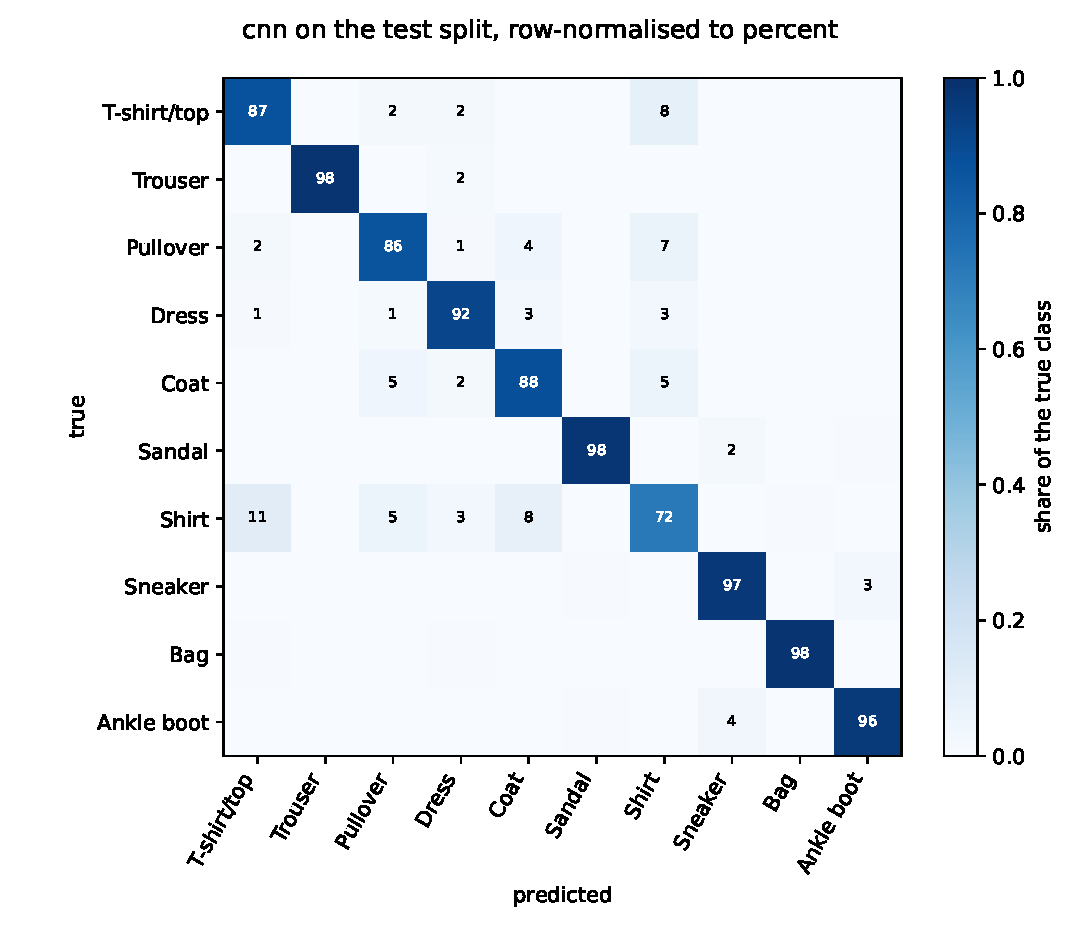
\includegraphics[width=0.8\textwidth]{images/confusion_cnn_test.pdf}
    \caption{Confusion matrix of the CNN on the test split, rows normalised to percent.}
    \label{fig:confusion}
\end{figure}

\begin{figure}[H]
    \centering
    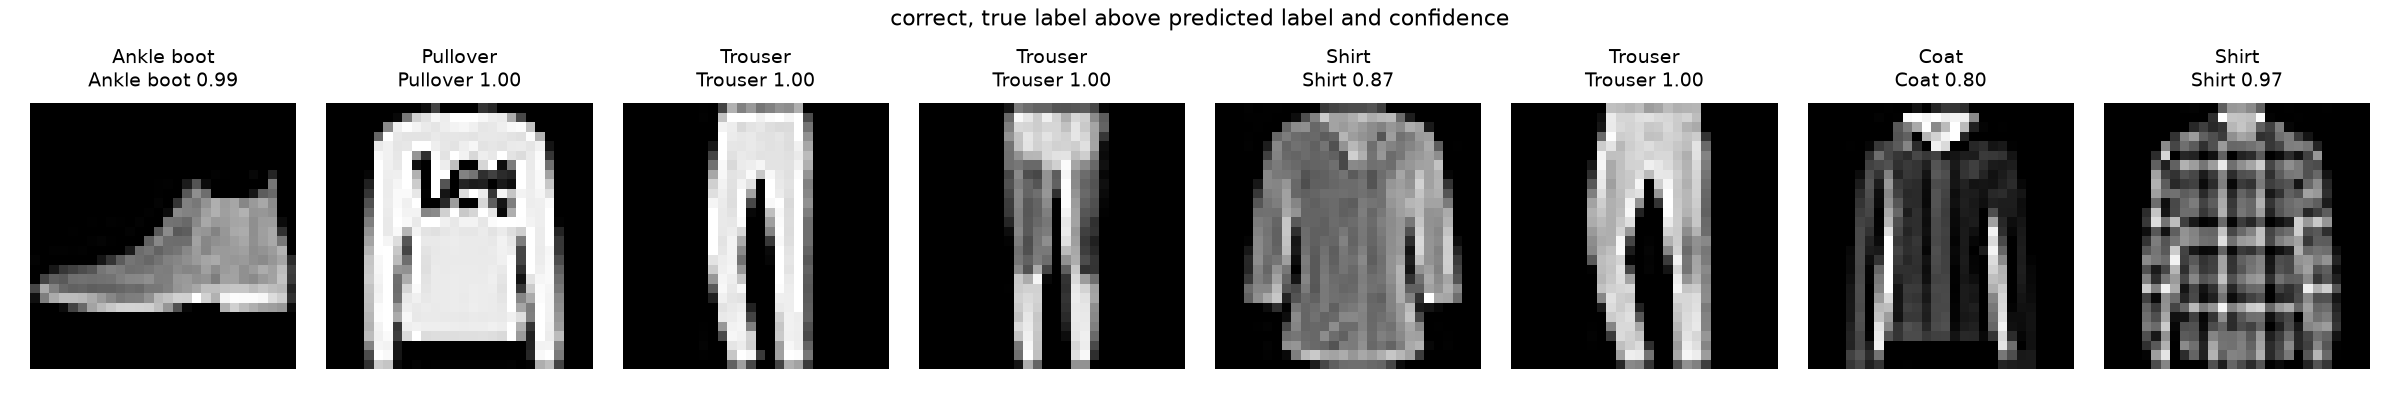
\includegraphics[width=\textwidth]{images/predictions_correct.png}

    \vspace{2mm}
    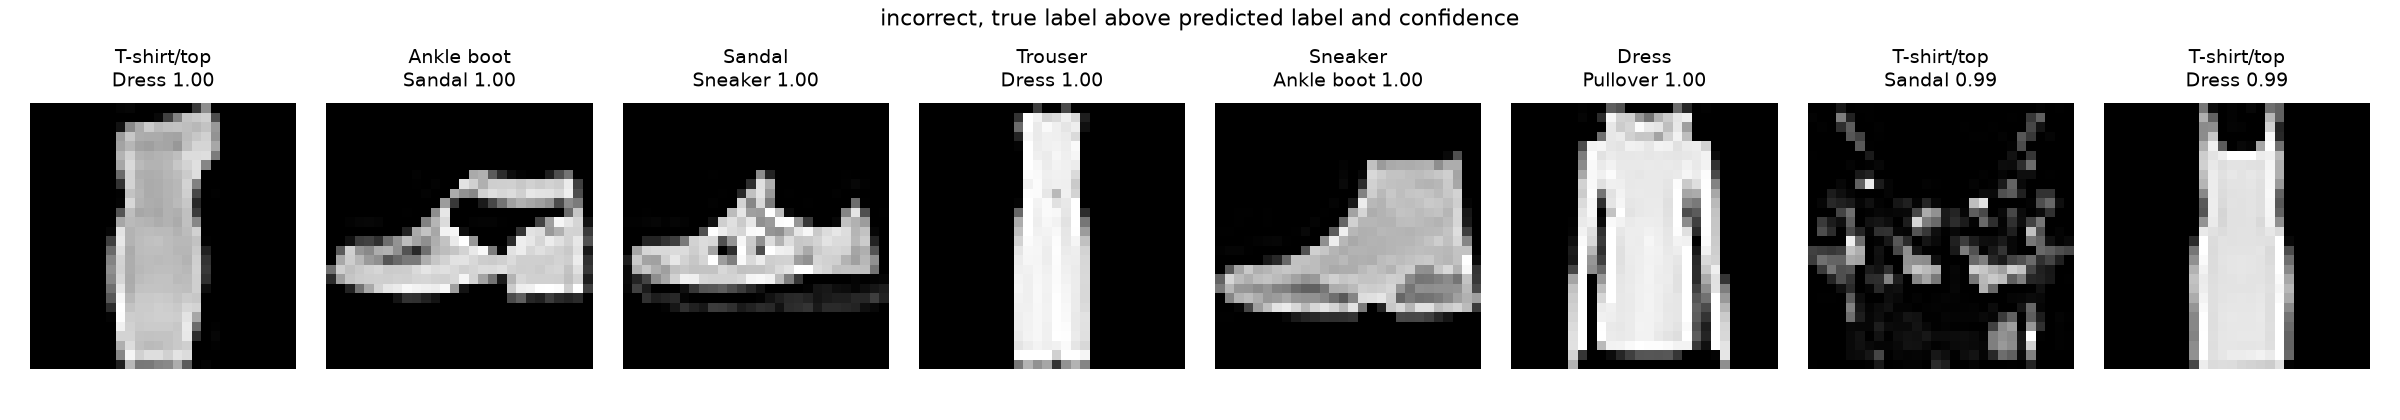
\includegraphics[width=\textwidth]{images/predictions_incorrect.png}
    \caption{CNN predictions on the test split: correct above, errors below.}
    \label{fig:predictions}
\end{figure}

Figure~\ref{fig:predictions} places predictions against ground truth: the upper row is the first
eight test images in loader order, the lower the eight errors the model was most confident about.
The upper row holds two genuinely difficult cases the model still resolves, a plaid Shirt at
confidence $0.97$ and a dark hooded Coat at $0.80$, both recognised from texture and silhouette
rather than brightness. The lower row is more informative, because every image in it fails at
confidence $0.99$ or above: a sleeveless garment labelled T-shirt/top but predicted Dress, a flat
open-backed shoe labelled Ankle boot but predicted Sandal, a Trouser predicted Dress. The model
is not uncertain about these; the image is simply compatible with both labels. They mark a
ceiling no architecture compared here can pass.

\subsection{Comparison and discussion}
\label{subsec:results-4}
% Required: Which method is better and by how much; where differences appear; causes in data, architecture, loss or training; accuracy, speed and parameter trade-offs; whether hypotheses are supported; conclusions that cannot yet be drawn. Listing metrics and declaring the highest score best is not sufficient.
% Also required: Section 12.1: analyse how data representation and inductive bias affect performance; do not conclude from accuracy alone. Section 12.2: same split and protocol for all models; report hardware, software versions, seeds, and the checkpoint selection rule.

Applying the criterion of Section~\ref{subsec:methodology-4} to Table~\ref{tab:results}, the CNN
beats all four alternatives, the MLP and the Transformer are indistinguishable from each other,
both beat the GRU, and all four beat the Linear baseline. The CNN's margin on test is $0.0303$
macro-F1 over the MLP and $0.1491$ over the baseline. The comparison is admissible because every
model saw the identical committed split under the protocol of Table~\ref{tab:protocol}, with the
same seeds, checkpoint rule, hardware and library versions.

The ranking does not follow capacity. The CNN wins with $21\%$ fewer parameters than the MLP and
$22\%$ fewer than the Transformer, and the Transformer, the largest and most expensive to train,
does not separate from an MLP that trains in half the time. What distinguishes the five is the
inductive bias each imposes on the same pixels, which follows from the input representation. The
CNN keeps the image as a grid and assumes locality and translation equivariance, matching the
pixel correlation of Section~\ref{subsec:problem-and-data-3}; the weight sharing this implies is
why it is at once the most accurate and the smallest of the three strong models. The MLP receives
a flat vector in which neighbouring pixels are no longer neighbours, so it learns that structure
from data and pays in parameters. The GRU sees rows in sequence, capturing real vertical
structure but asserting a processing order a static image does not have. The Transformer has no
locality prior, so attention must discover neighbourhood relations from data, and at this scale
it does not close the gap. The baseline's $0.7619$ measures directly that the classes are not
linearly separable in pixel space.

Accuracy is not the only axis. The GRU reaches $0.8667$ with under an eighth of the MLP's
parameters, trailing it by $0.0140$, yet is slowest at inference, $2.069$~ms per image against
the CNN's $0.305$, because its timesteps are sequential while convolution is not; parameters and
latency are not interchangeable proxies for cost. Among the models competitive on accuracy the
CNN is also the cheapest to run, so here there is no accuracy-against-speed trade-off.

The hypothesis that inductive bias rather than capacity governs performance is therefore
supported, but two conclusions do not follow. The first is that attention is the reason the
Transformer trails: the ablation of Section~\ref{subsec:results-6} shows that most of its deficit
against the MLP comes from the patch tokenisation it was given, not from the architecture, and
that the same model on row tokens beats the MLP outright. The attribution above therefore holds
for the Transformer only as configured here. The second
is that any single component of the CNN causes its advantage; separating locality from weight
sharing from pooling would need a further ablation that was not run.

\subsection{Error analysis}
\label{subsec:results-5}
% Required: Per error group: description; frequency or rate if possible; examples; hypothesized cause; improvement ideas.

The CNN misclassifies $888$ of the $10{,}000$ test images, an error rate of $8.9\%$ averaged over
three seeds. Table~\ref{tab:error-groups} splits them into three groups of very unequal size.

\begin{table}[H]
\centering
\caption{Error groups for the CNN on the test split.}
\label{tab:error-groups}
\begin{tabularx}{\textwidth}{lrrX}
\hline
\textbf{Group} & \textbf{Errors} & \textbf{Share} & \textbf{Description} \\
\hline
Upper-body garments & 576 & 64.9\% & Confusions among T-shirt/top, Pullover, Coat and Shirt \\
Footwear            &  93 & 10.5\% & Confusions among Sandal, Sneaker and Ankle boot \\
Scattered           & 219 & 24.6\% & Remainder, of which $81\%$ involve Dress \\
\hline
Total               & 888 & 100\% & \\
\hline
\end{tabularx}
\end{table}

\textbf{Upper-body garments.} Almost two thirds of all errors, every confusion bidirectional. The
largest flows are Shirt predicted as T-shirt/top, $118$ of $1{,}000$ Shirts, then T-shirt/top as
Shirt, $78$, and Shirt as Coat, $75$. Shirt is the only class below $0.80$ F1, at $0.7365$ with
precision $0.753$ and recall $0.721$, and it is the lowest class for all five architectures. The
cause lies in the data: these classes are separated by sleeve length, collar shape and fabric
texture, and Figure~\ref{fig:overlap} showed before any training that they have the most similar
class means. The same block holds $64\%$ of the MLP's errors, $64\%$ of the GRU's, $61\%$ of the
Transformer's and $48\%$ of the Linear baseline's, so it is a property of the task at this
resolution rather than of any one architecture. The baseline is the exception that confirms it:
its errors are the least concentrated only because it also makes $2{,}369$ of them, spreading
failure over classes the other four separate easily.

\textbf{Footwear.} Only $93$ errors across three close classes. Sole shape and ankle height
survive downsampling far better than fabric texture, which is why all three exceed $0.95$ F1 and
why this group is not worth attacking.

\textbf{Scattered errors.} The remaining quarter is spread thinly and dominated by Dress,
involved in $81\%$ of it, chiefly against Shirt and Coat. It includes the confident failures of
Figure~\ref{fig:predictions}, where the annotation is arguably as much at fault as the
prediction.

Only the first group is worth improving, and capacity is not the way: the Transformer carries
$28\%$ more parameters than the CNN and a worse Shirt F1. A class-weighted or focal loss would
trade precision on the three easier classes for recall on Shirt, where macro-F1 is lost.
Augmentation targeted at sleeve and collar geometry would make the separating cues more salient
than a random crop does. A second-stage classifier on the four-class block would specialise on
the $65\%$ of errors that matter.

\subsection{Ablation study}
\label{subsec:results-6}
% Required: Mandatory for Assignments 2 and 3; recommended for Assignment 1 when comparing representations or regularizers.
% Also required: Section 3.3: recommended for Assignment 1 when comparing representations or regularizers.

The comparison above gives each sequence model its own default view of the image, so it
confounds the architecture with that view. Two ablations separate them. Both hold the protocol of
Table~\ref{tab:protocol} and the three seeds fixed, both are judged on validation by the
criterion of Section~\ref{subsec:methodology-4}, and the test split is not touched.

\subsubsection{Sequence representation}
\label{subsubsec:ablation-representation}

The first ablation fixes the architecture and varies only how the image is turned into a
sequence: $28$ rows of $28$ features, $28$ columns of $28$, or $49$ patches of $16$.
Table~\ref{tab:ablation-representation} and Figure~\ref{fig:ablation} report the result.

\begin{table}[H]
\centering
\caption{Sequence representation.}
\label{tab:ablation-representation}
\begin{tabular}{llrrrr}
\hline
\textbf{Model} & \textbf{Representation} & \textbf{Tokens} & \textbf{Parameters} & \textbf{s/epoch} & \textbf{Val macro-F1} \\
\hline
GRU         & rows                  & $28 \times 28$ & 62{,}218 & 14.7 & $\mathbf{0.8731 \pm 0.0012}$ \\
GRU         & columns               & $28 \times 28$ & 62{,}218 & 14.6 & $0.8726 \pm 0.0017$ \\
GRU         & $4 \times 4$ patches  & $49 \times 16$ & 57{,}610 & 17.8 & $0.8215 \pm 0.0007$ \\
\hline
Transformer & rows                  & $28 \times 28$ & 539{,}018 & 18.4 & $\mathbf{0.8987 \pm 0.0024}$ \\
Transformer & columns               & $28 \times 28$ & 539{,}018 & 18.4 & $0.8961 \pm 0.0014$ \\
Transformer & $4 \times 4$ patches  & $49 \times 16$ & 540{,}170 & 23.0 & $0.8834 \pm 0.0023$ \\
\hline
\end{tabular}
\end{table}

The hypothesis that patch tokens would win, because a patch preserves two-dimensional locality,
is refuted for both architectures: patches are the worst of the three every time. Rows and
columns are indistinguishable from each other, which is expected, since these garments are
roughly symmetric about the vertical axis and neither scan direction sees more structure than
the other.

\begin{figure}[H]
    \centering
    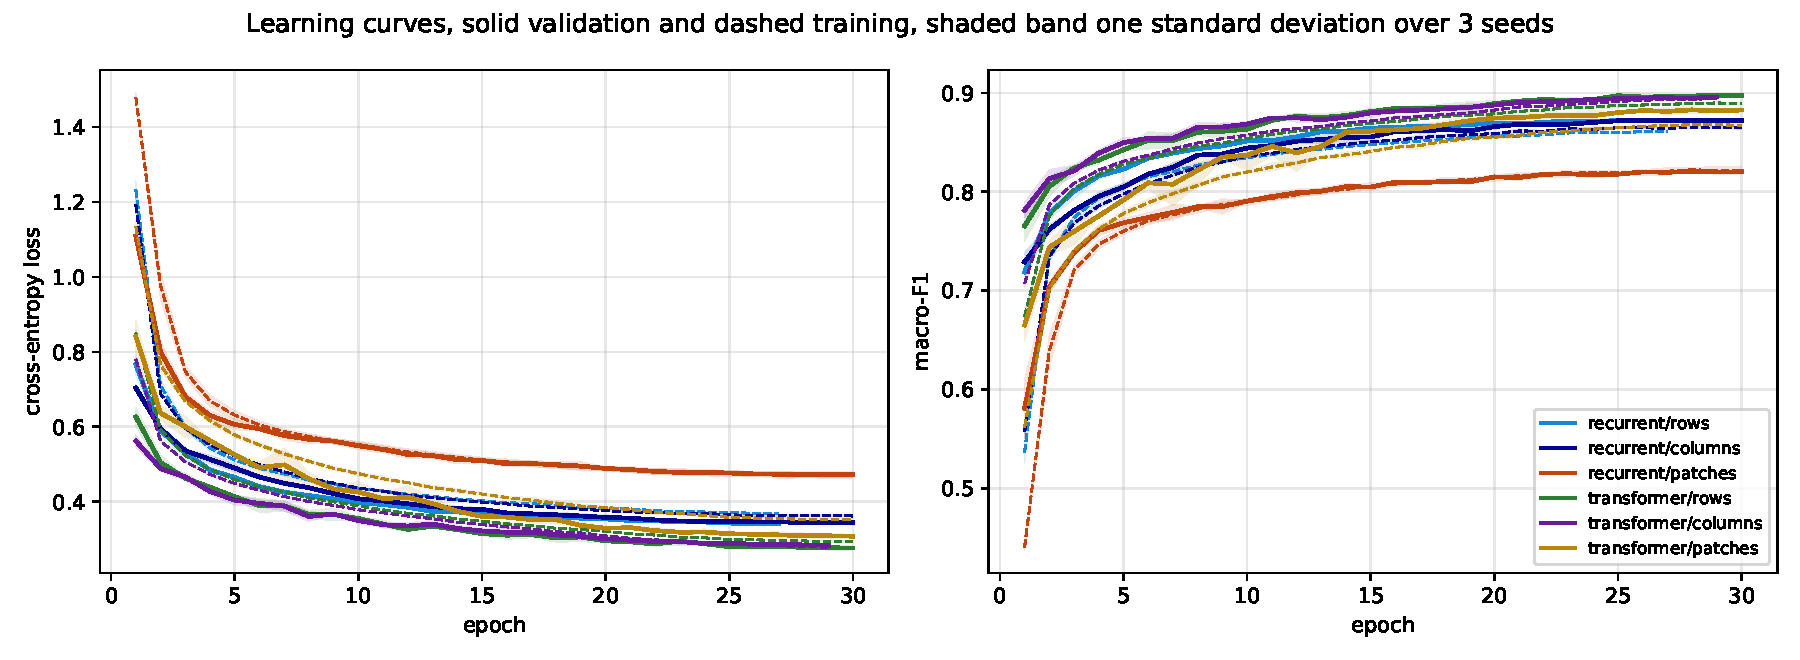
\includegraphics[width=\textwidth]{images/ablation_representation.pdf}
    \caption{Learning curves for the six representation configurations.}
    \label{fig:ablation}
\end{figure}

Figure~\ref{fig:sequences} explains why. Three patch tokens fall below a quarter of peak signal
against no row, because patch tokenisation gathers the empty border into a few near-constant
tokens; a patch sequence carries the same information in more tokens, each narrower and several
nearly empty. The cost is very unequal, $-0.0516$ macro-F1 for the GRU against $-0.0153$ for the
Transformer, and the asymmetry follows from how each reaches distant information. Attention
addresses any token directly, so lengthening the sequence from $28$ to $49$ costs it little,
whereas recurrence carries state across every added step, and $75\%$ more steps of a weaker
signal is where the GRU loses. Patches are also slower for both, because sequence length sets the
number of sequential steps.

\subsubsection{Recurrent cell}
\label{subsubsec:ablation-cell}

The second ablation fixes the row representation and varies only the gating, between the GRU used
throughout and an LSTM of the same hidden size and depth.

\begin{table}[H]
\centering
\caption{Recurrent cell at the row representation.}
\label{tab:ablation-cell}
\begin{tabular}{lrrrrr}
\hline
\textbf{Cell} & \textbf{Parameters} & \textbf{s/epoch} & \textbf{ms/image} & \textbf{Val macro-F1} & \textbf{Val accuracy} \\
\hline
LSTM & 82{,}442 & 12.7 & 0.630 & $\mathbf{0.8767 \pm 0.0011}$ & $\mathbf{0.8773 \pm 0.0013}$ \\
GRU  & 62{,}218 & 14.7 & 2.180 & $0.8731 \pm 0.0012$ & $0.8734 \pm 0.0014$ \\
\hline
\end{tabular}
\end{table}

The hypothesis that the GRU would match the LSTM at lower capacity is refuted on both counts, as
Table~\ref{tab:ablation-cell} shows. The LSTM is better, by $0.0036$ macro-F1 with
non-overlapping intervals, and cheaper to run despite $33\%$ more parameters. The margin is small
and bought with those parameters, so it says only that the separate cell state helps slightly
over $28$ steps. The timing should be read with care: an LSTM does strictly more arithmetic per
step, so the $14\%$ faster epoch and $3.5\times$ faster inference are properties of how well each
fused kernel is optimised on this backend, not of the algorithms, and nothing here measures the
kernels directly.

\subsubsection{Effect on the main comparison}
\label{subsubsec:ablation-effect}

The representation ablation revises one conclusion of Section~\ref{subsec:results-4}. On row
tokens the Transformer reaches $0.8987 \pm 0.0024$, whose interval clears the MLP's
$0.8862 \pm 0.0015$, so the two are no longer indistinguishable: the Transformer beats the MLP
once it is given a representation that suits it. The tie reported in Table~\ref{tab:results} is
thus an artefact of the patch tokenisation, not evidence that attention cannot exceed a dense
network at this scale.

What survives unchanged is the headline. The CNN at $0.9198 \pm 0.0018$ still beats the best
sequence configuration found here by a clear margin, with fewer parameters than either sequence
model, so inductive bias rather than capacity remains the better explanation of the ranking. The
GRU's choice of rows, made before these experiments, also turns out to have been its best
option.

\subsection{Limitations and conclusion}
\label{subsec:results-7}
% Required: Data, method and experimental limits; generalization; future work; short answer to the research question.

Four limits bound these results. The comparison uses one dataset of $28 \times 28$ grayscale
images with balanced classes, so neither the ranking nor the error structure should be assumed to
carry over to natural images, higher resolutions or imbalanced data. Three seeds estimate a
standard deviation from three observations, so a tie means two configurations were not separated
at this sample size, not that they are equal. All five share one optimizer, schedule and budget,
as fairness demands, so each figure is a score under a common protocol rather than the best each
architecture could reach. No pretrained weights are used, which constrains the Transformer
most.

The research question was whether architectural inductive bias or capacity governs performance
here. The evidence favours inductive bias: the most accurate model is the smallest of the three
strong ones, it keeps its margin even over the best sequence configuration the ablations found,
and the error structure dominating every residual was predicted from the class means before any
network was trained. The CNN is carried forward at $0.9110 \pm 0.0007$ macro-F1 on test.

The ablations also show how much a result can depend on a choice made before any measurement:
the Transformer's apparent tie with the MLP was an artefact of its default tokenisation, and
disappeared once the representation was varied. That is the clearest direction for further work,
since only two of the five architectures were ablated this way and the remaining three were never
compared at more than one view of their input. The other direction is a loss reweighted towards
Shirt, the one class that bounds macro-F1 for all five models.
